\documentclass{article}
\usepackage[utf8]{inputenc}
\usepackage{graphicx}

\title{\Huge Comptes rendus réunions n°4}
\author{Ridel Julien - Youssef Trabelsi - François Denes \\ Durée : 1h20}
\date{25/11/2021}

\usepackage{natbib}
\usepackage{graphicx}

\begin{document}

\maketitle

\section{\huge Objectifs de la séance}

\Large Procéder au découpage de notre projet en lots selon le système WBS et début de mise en place d'un matrice RACI

\section{\huge Contenu de la réunion } 
\Large Nous nous sommes réunis afin de découper notre projet en lots. Avec l'aide du site internet draw.io, nous avon pu créer un arbre représentant l'ensemble des taches à réaliser lors de notre projet. Puis, à l'aide de cet arbre, nous avons commencé à réaliser une matrice RACI afin de répartir les tâches entre les personnes du groupe. La matrice RACI n'a pas été terminée, mais l'arbre des lots est présenté ci-dessous. Le fichier draw.io sera présent dans le répertoire de ce compte rendu pour avoir l'arbre en entier\\

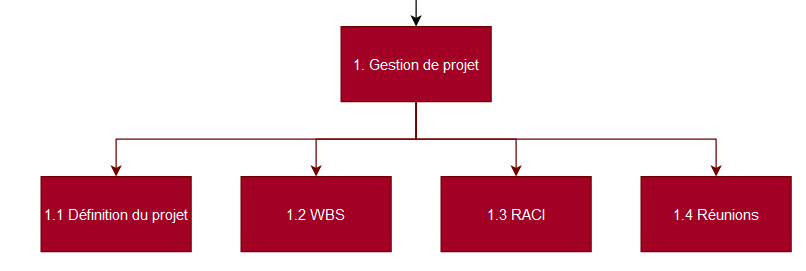
\includegraphics[scale=0.75]{1.png} \\
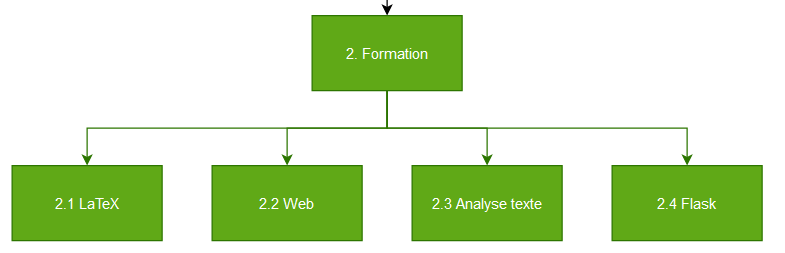
\includegraphics[scale=0.75]{2.png} \\
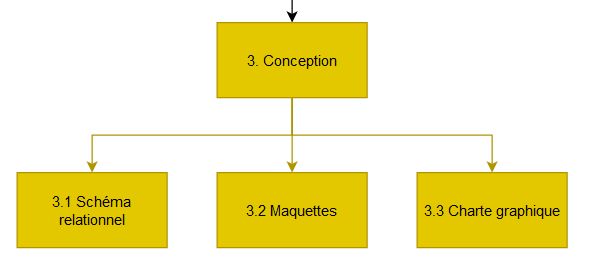
\includegraphics[scale=0.75]{3.png} \\
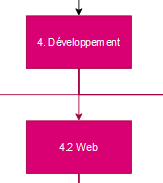
\includegraphics[scale=0.75]{4.png} 
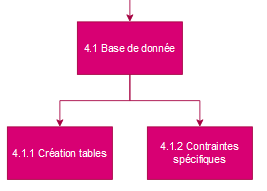
\includegraphics[scale=0.75]{5.png} 
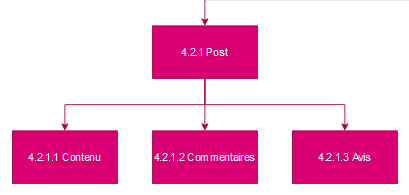
\includegraphics[scale=0.75]{6.png} \\
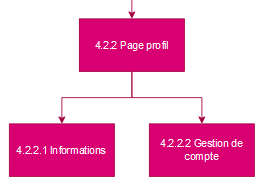
\includegraphics[scale=0.75]{7.png} 
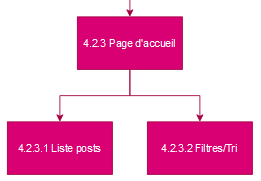
\includegraphics[scale=0.75]{8.png} 
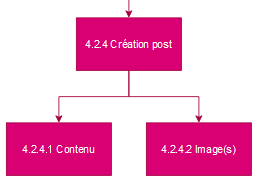
\includegraphics[scale=0.75]{9.png} \\
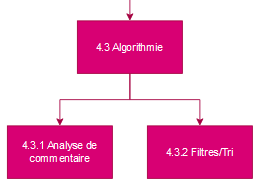
\includegraphics[scale=0.75]{10.png} 
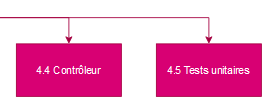
\includegraphics[scale=0.75]{11.png} \\ 
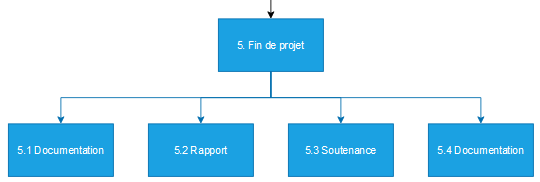
\includegraphics[scale=0.75]{12.png} \\

\end{document}
